
\documentclass[12pt]{article} 
\usepackage[utf8]{inputenc}
\usepackage[slovak]{babel}
\usepackage[hidelinks,unicode = true]{hyperref}
\usepackage{outline}
\usepackage{graphicx}
\usepackage{longtable} %pro tabulky delší než jedna stránka
%\usepackage{biblatex}
%\addbibresource{literatura.bib}
\usepackage{cite}
\usepackage{caption}
%\usepackage{float} %upevneni tabulky
%\restylefloat{table}
\setcounter{secnumdepth}{3}
\setcounter{tocdepth}{3}

%===========================================================================
\begin{document}           % Konec preambule a zároveň začátek vlastního textu
\begin{titlepage}
\centering
\Large \textbf{České vysoké učení technické v Praze }\\ Fakulta stavební
\vspace{2cm}

\begin{figure}[h!] %logoCVUT
\centering
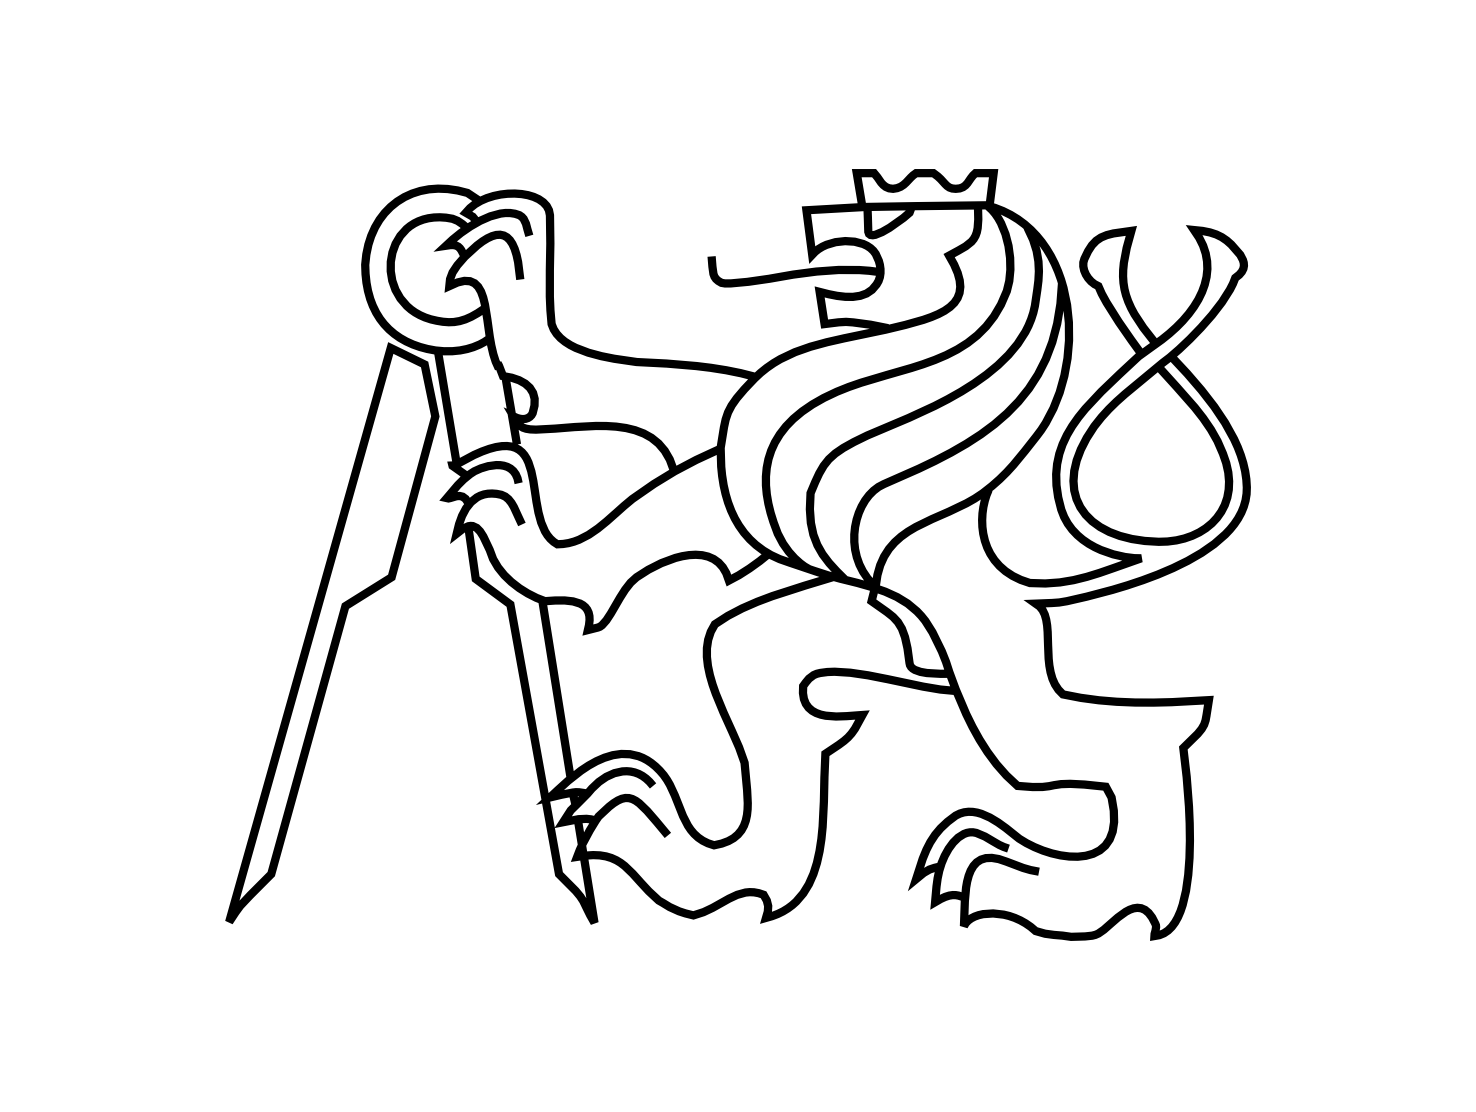
\includegraphics[width=7cm]{./img/cvut.png}
\end{figure}
 
\Large \textbf{155ADKG Algoritmy v digitální kartografii}
\vspace{1cm}

\LARGE  \textbf{ Digitální model terénu a jeho analýzy}
\vspace{3cm}

\Large Bc. Lukáš Kettner Bc. Martin Hulín \\ 1.12.2019

 \thispagestyle{empty} %neočísluje první stránku
\end{titlepage}

\tableofcontents    % vytváří  Obsah 
\newpage %začne na nové stránce
%------------------------------------------------------------------------
\section{Zadanie}
Vytvorte aplikáciu s grafickým rozhraním, ktorá vygenerujedigitálny model terénu. Vstup do aplikácie : množina bodov P = \{p1, …, pn\},  p{i} = \{x{i}, y{i}, z{i}\} .
\newline Výstup aplikácie : polzedrický DMT nad množinou P reprezentovaný vrstevnicami, ktorý je doplnený vizualizáciou sklonu trojuholníkov a ich expozíciou  \textit{H}(P).

Metódou inkrementálnej konštrukcie vytvorte nad množinou   \textit{P} vstupných bodov 2D Delaunay trianguláciu. Ako vstupné dáta použite existujúce geodetické dáta (minimálne 300 bodov) alebo navrhnite algoritmus pre generovanie syntetických vstupných dát, ktoré budú predstavovať významné terénne tvary (kopa, odpočinok, chrbát, údolie, atď. ).

Nad vzniknutou trianguláciou vygenerujte DMT a prevedte analýzy :

\begin{itemize}
\item Vizualizáciu s rozlíšením zvýraznených vrstevníc 
\item Analyzujte sklon DMT, jednotlivé trojuholníky vizualizujte v závislosti na sklone
\item Analyzujte expozíciiu DMT, jednotlivé trojuholníky vizualizujte v závislosti na ich expozícii ku svetovej strane 
\end{itemize}
		
Zhodnoťte výsledný DMT z kartografického hladiska. Uvážte prípady, kedy 2D Delaunay triangulácia nebude dávať vhodné výsledky.

\subsection{Bonusové úlohy}
V rámci úlohy sú vypracované tieto bonusové úlohy

\begin{itemize}
\item Automatický popis vrstevnic
\item Výber farebných stupníc pre vizualizáciu sklonu a expozície
\item Algoritmus pre automatické generovanie terénnych tvarov
\end{itemize}
%------------------------------------------------------------------------
\clearpage 
\section{Popis a rozbor problému}
Problematika úlohy sa týka tvorby digitálneho modelu terénu. Pri vstupe máme zadanú množinu bodov P = \{p1, …, pn\},  p{i} = \{x{i}, y{i}, z{i}\} . Nad touto množinou je potrebné vytvoriť trojuholníkovú sieť. Túto sieť je potrebné vytvárať pomocou Delaunay triangulácie. Po korektnom vyvorení triangulačnej siete je potrebné vygenerovať vrstevnice ,určiť sklon digitálneho modelu terénu a expozíciu jednotlivých trojuholníkov triangulácie.

\begin{center}
   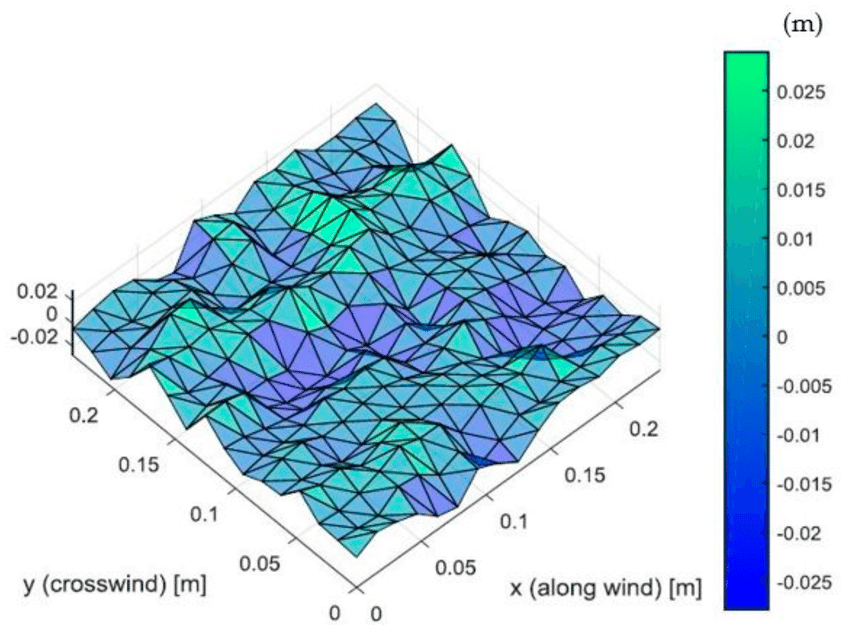
\includegraphics[width=12cm]{./img/Delaunay_DTM.png}
   \captionof{figure}{3D model vodného povrchu vytvorený pomocou Delaunay triangulácie}
\end{center}

%------------------------------------------------------------------------
\clearpage 
\section {Popis použitých algoritmov}
\subsection {Delaunay triangulácia}
Tento algoritmus predstavuje jeden z najpoužívanejích postupov pre tvorbu digitálneho modelu terénu. Triangulácia je realizovaná metódou inkrementálnej konštrukcie. V algoritme sa zavádza kritérium postupného hladania bodu, ktorý k bodom hrany vytvorí minimálnu opísanú kružnicu. Takýto bod sa vždy hľadá v ľavej polorovine orientovaných hran. 

\subsubsection {Vlastnosti Delaunay triangulácie}
\begin{enumerate}
\item Vnútri písanej kružnice každého trojuholníku sa nenachádza žiadny iný bod
\item Maximalizuje minimálny uhol v trojuholníku
\item Je lokálne aj globálne optimálna voči kritériu minimálneho uhlu
\item Je jednoznačná, pokiaľ na kružnici ležia 3 body
\end{enumerate}

\subsubsection{Implementácia metódy}



\begin{enumerate}
\item Zoraď vstupnú množinu bodov podľa súradnice X
\item Nájdi bod $p_1$ s minimálnou súradnicou X 
\item Nájdi najbližší bod$ ||p_1-q|| = min $ 
\item Vytvor hranu $ e = (p_1,p_2) $ 
\item  Nájdi Delaunay bod :  $p_{min} = arg min_{\forall p_i\in\sigma_L(e)} r'(k_i), k_i = (a, b, p_i), e = (a,b)$
\item \hspace {1.5cm} Pokiaľ taký bod nie je nájdený, zmeň orientáciu a opakuj hľadanie
\item Vytvor zvyšné hrany trojuholníku $e_2 = (p_1,p_{min}), e_3 = (p_{min},p_1) $
\item  Pridanie hrán do AEL $ AEL \leftarrow e, AEL  \gets e_2,  AEL \gets e_3 $
\item  Pridanie hrán do DT $ DT \gets e, DT \gets e_2,  DT \gets e_3 $
\item  Pokiaľ AEL nie je prázdny :
\item \hspace {1cm} Vezmi prvú hranu z	 AEL $AEL  \longrightarrow e, e = ( p_1, p_2) $
\item \hspace {1cm} Prehoď orientáciu tejto hrany $ e = (p_2, p_1)$ 
\item \hspace {1cm} $p_{min} = arg min_{\forall p_i\in\sigma_L(e)} r'(k_i), k_i = (a, b, p_i), e = (a,b) $
\item \hspace {1cm} Ak existuje takýto bod if $ \exists p_{min}:$
\item \hspace {1.5cm} Vytvor zvyšné hrany trojuholníku $e_2 = (p_1,p_{min}), e_2 = (p_{min},p_1)  $
\item \hspace {1.5cm} Pridaj hranu do DT, no nie do AEL $DT \longleftarrow e  $  
\item \hspace {1.5cm} $ add(e_2,AEL,DT), add(e_3,AEL,DT)$
\end{enumerate}

\subsubsection {Problematické situácie}
Problematickou situáciou sú .....

\subsection {Vrstevnice}
Algoritmus pre generovanie vrstevníc využíva lineárnu interpoláciu. Pri lineárnej interpolácii sa predpokladá konštantný spád medzi podrobnými bodmi $p_i$.

\subsubsection{Implementácia metódy}
\begin{enumerate}
\item Pre všetky hrany trojuholníku platí:
\item Hrana patrí rovine vrstevnice  $(z-z_i)*(z-z_{i+1}) < 0$  $\longrightarrow e_i \cap \rho$
\item Hrana nepatrí rovine vrstevnice $(z-z_i)*(z-z_{i+1}) > 0$  $\longrightarrow e_i \notin \rho$ 
\item Hrana je prienikom roviny vrstevnice $(z-z_i)*(z-z_{i+1}) = 0$  $\longrightarrow e_i \in \rho$
\item  \hspace {1.5cm} Výpočet súradníc priesečníku 
\item  \hspace {1.5cm} $$ x = \frac{(x_2-x_1)}{(z_2-z_1)}(z-z_1)+x_1, $$
\item  \hspace {1.5cm} $$ y = \frac{(y_2-y_1)}{(z_2-z_1)}(z-z_1)+y_1.$$
\item Vytvor hranu, ktorá tvorí vrstevnicu
\end{enumerate}

\subsection {Sklon terénu}
Analýza sklonu terénu je jednou z najčastejších úloh vykonávaných nad DMT. Využíva sa v rozličných oblastiach pre analýzu odtoku sedimentov, zosuvu pôdy, či projektovania líniových stavieb. Sklon je definovaný ako uhol medzi normálovým vektorom a normálovým vektorom trojuholníka. Pre jeho výpočet je potrebné spočítať smerové vektory v trojuholníkoch. Normálový vektor (0, 0, 1) má normu o veľkosti 1. Tým pádom vo funkcii arccos zostáva len z-ová časť normálového vektoru. Sklon sme vyzualizovali v odtieňoch šedi a odtieňoch základných farieb RGB.

\subsubsection{Implementácia metódy}
n = (0,0,1)
\newline $n_t = \vec{u}\times \vec{v}$
$$\varphi =\arccos(\frac{n_t \cdot n}{|n_t| |n|})$$

\subsection {Expozícia}
Expozícia je definovaná ako orientácia jednotlivých trojuholníkov k svetovým stranám.

\subsubsection{Implementácia metódy}
\begin{enumerate}
	\item Pre všetky trojuholníka triangulácie vypočítaj : 
	\item X a Y zložku normálového vekotu $ n_x = (u_y * v_z - u_z * v_y) , n_y = - (u_x * v_z - u_z * v_x) $
	\item Výpočet expozície $$A = \arctan2(\frac{n_x}{n_y});$$

\end{enumerate}

\clearpage 
%------------------------------------------------------------------------
\section{Bonusové úlohy}

\subsection {Automatické generovanie terénnych tvarov }
.

\subsection{Automatický popis vrstevnic}
Do pôvodneho algoritmu pre výpočet vrstevníc sme zakomponovali vektor metadat, do ktorého sa ukladala výška vrstevnice. Následne z tohto vektoru boli pre hlavné vrstevnice pridané výškové informácie. Tento spôsob nie je v súhlade s katografickými zásadami (orientácia, vhodné rozmiestnenie a umiestnenie výškových kót). Pri určitých typoch terénu sa popis vrstevnice zobrazí mnohonásobne a tým znemožní správnu vyzualizáciu hlavnej vrstevnice. Riešením by bola úprava algoritmu tak aby rešpektoval kartografické zásady. Mohlo by to byť dosiahnute implementáciou bufferu , prepojením algoritmusu pre výpočet sklonu s algoritmom výpočtu a vykreslenia vrstevníc, či obmedzením na počet vykreslovania popisu vrstevníc. Vzhladom na časové možnosti autorov aplikácie nebol tento problém riešený

\subsection{Výber farebných stupníc pre vizualizáciu sklonu a expozície}
V rámci bonusových úloh bola riešená možnosť výberu farebných stupníp pre analýzu sklonu a expozície. Užívateľ má pre analýzu sklonu na výber zo základných farieb RGB (červená, zelená, modrá) alebo základnú šedú farbu. Skon je následne vizualizovaný v odtieňoch vybranej farby. Pre analýzu expozície má užívateľ k dispozícii 5 farebných stupníc. Defaultna farebná stupnica je vytvorená podľa stupnice programu Argis Pro. Ďalšie tri stupnice sú v sýtych farbách, odstupňované podľa rozsahu veľkosti sklonu na danom území. Poslednou stupnicou je takzvaná Sun color stupnica, ktorá zobrazuje orientáciu k svetovým stranám na základe  ,,intuitívnej" farby slnka ( sever - biela, východ - žltá, juh - červená, západ - oranžová).


%------------------------------------------------------------------------
\clearpage 
\section{Vstupné data}
Vstupnými dátami pre tvorbu DMT sú body so súradnicami Y, X, Z. Tieto body je možné v aplikácii ručne naklikať, automaticky vygenerovať alebo nahrať vo formáte *.txt . Súbor, ktorý užívateľ chce importovať do aplikácie musí byť vo formáte Y, X, Z bez čísla bodu.


\begin{center}
   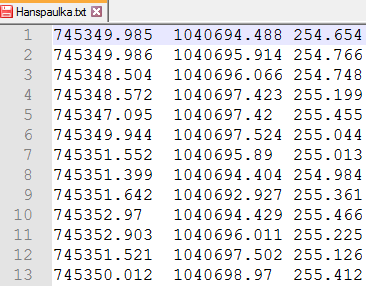
\includegraphics[width=10cm]{./img/vstupny_format.png}
   \captionof{figure}{Ukážka vstupného formátu súradníc}
\end{center}


%-------------------------------------------------------------------------
\clearpage 
\section{Výstup aplikácie}


%-------------------------------------------------------------------------

\section{Dokumentácia}
\subsection{Trieda Algorithms}
Triedu Algorithms sme použili pre deklarovanie funkcií pre výpočtové algoritmy tvorby DMT.

\subsubsection{Metódy}
\begin{enumerate}
\item[] \underline{getPointLinePosition}
\begin{itemize}
\item je pomocnou metódou pre metódu positionPointPolygonWinding. Slúži na určenie polohy bodu voči priamke. Jej návratovou hodnotou je integer.
\item na vstupe má : súradnice určovaného bodu q , súradnice bodov priamky $p_1$ $p_2$
\item na výstupe hodnoty :
\item[] -1 – bod sa nachádza na priamke
\item[] 0 – bod sa nachádza vpravo od priamky
\item[] 1 – bod sa nachádza vľavo od priamky
\end{itemize}

\item[] \underline{getCircleRadius}
\begin{itemize}
\item Slúži na výpočet polomeru kružnice tvorenej troma vstupnými bodmi. Návratová hodnota je double.
\item na vstupe má : súradnice troch bodov $p_1$, $p_2$ , $p_3$
\item na výstupe hodnotu polomeru kružnice.
\end{itemize}

\item[] \underline{getNearestPoint}
\begin{itemize}
\item Slúži na nájdenie najbližšieho indexu k bodu p. 
\item na vstupe má : súradnice bodu  $p$  a vektor bodov.
\item na výstupe má index najbližšieho bodu k bodu p.
\end{itemize}

\item[] \underline{getDistance}
\begin{itemize}
\item Slúži na výpočet vzdialenosti medzi dvom bodmi. Návratová hodnota je double. 
\item na vstupe má : súradnice bodov medzi ktorými počítame vzdialenosť.
\item na výstupe má vzdialenosť medzi bodmi.
\end{itemize}

\item[] \underline{getDelaunayPoint}
\begin{itemize}
\item Slúži na nájdenie indexu bodu, ktorý spĺňa podmienky Delaunay triangulácie. 
\item na vstupe má : súradnice bodov začiatku a koncu hrany, vektor bodov
\item na výstupe index bodu, ktorý spĺňa podmienky Delaunay triangulácie.
\end{itemize}

\item[] \underline {std::vector}$<${Edge}$>${DT}
\begin{itemize}
\item Metóda vytvára nad vektorom hran Delaunay trianguláciu.
\end{itemize}

\item[] \underline{QPoint3D getContourPoint}
\begin{itemize}
\item Metóda slúžia k výpočtu priesečníku hrany a rovinou Z. Vstupným typom je QPoint3D.
\item na vstupe sú súradnice bodov 3D hrany p1 a p2, rovina definovaná z súradnicou 
\item na výstupe sú súradnice priesečníka.
\end{itemize}

\item[] \underline {std::vector}$<${Edge}$>${createContours}
\begin{itemize}
\item Metóda slúži k výpočtu vrstevníc.
\item na vstupe sú vektor hran, rozsah vrstevníc (min/max) a ich krok, vektor metadát do ktorých sa ukladá informácia o výške vrstevnice
\item na výstupe je vektor hran vrstevníc.
\end{itemize}

\item[] \underline{getSlope}
\begin{itemize}
\item Slúži na výpočet sklonu trojuholníku, ktorý spĺňa podmienky Delaunay triangulácie. Návratovým typom je double.
\item na vstupe má : súradnice bodov trojuholníku.
\item na výstupe hodnotu sklonu.
\end{itemize}

\item[] \underline{getAspect}
\begin{itemize}
\item Slúži na výpočet orientácie / expozície trojuholníku, ktorý spĺňa podmienky Delaunay triangulácie. Návratovým typom je double.
\item na vstupe má : súradnice bodov trojuholníku.
\item na výstupe hodnotu expozície.
\end{itemize}

\item[] \underline {std::vector}$<${Triangle}$>${analyzeDMT}
\begin{itemize}
\item Metóda slúži k výpočtu trojuholníkov Delaunay triangulácie, k výpočtu ich sklonu a expozície. Návratovým typom je vektor trojuholníkov.
\item na vstupe je vektor hran Delaunay triangulácie
\item na výstupe je vektortrojuholníkov Delaunay triangulácie, sklon, expozícia.
\end{itemize}

\item[] \underline {std::vector}$<${QPoint3D}$>${importMeasurement}
\begin{itemize}
\item Metóda slúži k importu *.txt súboru obsahujúceho súradnice Y, X, Z 
\end{itemize}

\item[] \underline {std::vector}$<${QPoint3D}$>${generateShapes}
\begin{itemize}
\item Metóda slúži ku generovaniu prírodných tvarov.
\end{itemize}

\end{enumerate}

\subsection{Trieda Draw}
Trieda Draw slúži ku grafickému vykresleniu všetkých premenných.

\subsubsection{Členské premenné}
\begin{enumerate}

\item[] \underline {std::vector}$<${QPoint3D}$>${points}
\begin{itemize}
\item vektor bodov 
\end{itemize}

\item[] \underline {std::vector}$<${Edge}$>${dt}
\begin{itemize}
\item vektor hran Delaunay triangulácie
\end{itemize}

\item[] \underline {std::vector}$<${Edge}$>${contours}
\begin{itemize}
\item vektor hran vrstevníc
\end{itemize}

\item[] \underline {std::vector}$<${double}$>${metadata}
\begin{itemize}
\item vektor metadat vrstevníc - výšok vrstevníc
\end{itemize}

\item[] \underline {std::vector}$<${Triangle}$>${dmt}
\begin{itemize}
\item vektor tvorený trojuholníkmi Delaunay triangulácie
\end{itemize}

\item[] \underline {int dz}
\begin{itemize}
\item rozostup vrstevníc
\end{itemize}

\item[] \underline {int colorScale}
\begin{itemize}
\item typ farebnej škály
\end{itemize}

\item[] \underline {bool aspect, slope}
\begin{itemize}
\item vykreslenie sklonu a expozície
\end{itemize}

\end{enumerate}


\subsubsection{Metódy}
\begin{enumerate}
\item[] \underline{paintEvent}
\begin{itemize}
\item slúži k vykresleniu naklikaných, načítaných  a vygenerovaných bodov, vykresleniu Delaunay triangulácie, sklonu, expozície a vrstevniciam. Návratovým typom je void.
\end{itemize}
\item[] \underline{void mousePressEvent}
\begin{itemize}
\item slúži k vykresleniu bodu  stlačením tlačidla myši, v okamihu stlačenia tlačidla na myši sa uložia súradnice bodu do vektoru points. Návratovým typom je void.
\end{itemize}
\item[] \underline{void clearPoints}
\begin{itemize}
\item slúži k vymazaniu množiny bodov. Návratovým typom je void.
\end{itemize}
\item[] \underline{void clearDT}
\begin{itemize}
\item slúži k vymazaniuDelaunay triangulácie. Návratovým typom je void.
\end{itemize}
\item[] \underline{void clearContours}
\begin{itemize}
\item slúži k vymazaniu vrstevníc. Návratovým typom je void.
\end{itemize}
\item[] \underline{void clearSlope}
\begin{itemize}
\item slúži k vymazaniu sklonu. Návratovým typom je void.
\end{itemize}
\item[] \underline{void clearAspect}
\begin{itemize}
\item slúži k vymazaniu expozície. Návratovým typom je void.
\end{itemize}

\item[] \underline{getPoints}
\begin{itemize}
\item slúži k vrátenie členskej premennej points
\end{itemize}

\item[] \underline{getDT}
\begin{itemize}
\item slúži k vrátenie členskej premennej dt
\end{itemize}

\item[] \underline{getDTSize}
\begin{itemize}
\item slúži k vrátenie veľkosti členskej premennej dt
\end{itemize}

\item[] \underline{setPoints}
\begin{itemize}
\item slúži k priradeniu členskej premennej points
\end{itemize}

\item[] \underline{setDt}
\begin{itemize}
\item slúži k priradeniu členskej premennej dt
\end{itemize}

\item[] \underline{setDMT}
\begin{itemize}
\item slúži k priradeniu členskej premennej dmt
\end{itemize}

\item[] \underline{setContours}
\begin{itemize}
\item slúži k priradeniu členských premenných contours, metadata,$ d_z $
\end{itemize}

\item[] \underline{setSlope , set Aspect}
\begin{itemize}
\item slúžia k vykreslovaniu sklonu a expozície
\end{itemize}

\item[] \underline{setColorScale}
\begin{itemize}
\item slúži k nastaveniu farebnej škály vykreslovania sklonu a expozície
\end{itemize}

\end{enumerate}

\subsection{Trieda Edge}
Je to definície datového typu Edge. Reprezentuje usporiadanú dvojicu vrcholov, ktoré tvoria orientovanú hranu (vrcholy sú počiatkom a koncom hrany).

\subsubsection{Členské premenné}
\begin{enumerate}

\item[] \underline {QPoint 3D s,e}
\begin{itemize}
\item začiatok hrany s , konies hrany e
\end{itemize}
\end{enumerate}

\subsubsection{Metódy}
\begin{enumerate}
\item[] \underline{getStart, getEnd}
\begin{itemize}
\item slúži k vráteniu počiatočného ú koncového bodu hrany
\end{itemize}
\item[] \underline{change Orientation}
\begin{itemize}
\item slúži k obráteniu orientácie hrany
\end{itemize}
\end{enumerate}

\subsection{Trieda QPoint3D}
Je to odvodená trieda od triedy QPointF. Pridali sme k nej výškovú súradnicu z. 

\subsubsection{Členské premenné}

\begin{enumerate}
\item[] \underline {double z}
\begin{itemize}
\item výšková súradnica z
\end{itemize}
\end{enumerate}

\subsubsection{Metódy}
\begin{enumerate}
\item[] \underline{setZ}
\begin{itemize}
\item slúži k priradeniu hodnoty do členskej premennej z
\end{itemize}
\item[] \underline{getZ}
\begin{itemize}
\item slúži k získaniu súradnice z
\end{itemize}
\end{enumerate}

\subsection{Trieda Triangle}
Je to definícia novovytvoreného datového typu Triangle. V tejto triede sa ukladá trojica vrcholov tvoriacich trojuholník, sklon a expozícia.

\subsubsection{Členské premenné}
\begin{enumerate}
\item[] \underline {QPoint3D p1, p2, p3}
\begin{itemize}
\item vrcholy trojuholníka
\end{itemize}
\item[] \underline {double slope, aspect}
\begin{itemize}
\item sklon a expozícia trojuholníka
\end{itemize}
\end{enumerate}

\subsubsection{Metódy}
\begin{enumerate}
\item[] \underline{Triangle}
\begin{itemize}
\item slúži k uloženiu trojuholníka definovaného bodmi p1, p2, p3, sklonu a expozície
\end{itemize}

\item[] \underline{metódy get}
\begin{itemize}
\item slúži k získaniu danej premennej
\end{itemize}

\item[] \underline{metódy set}
\begin{itemize}
\item slúži k priradeniu hodnoty k danej premennej
\end{itemize}
\end{enumerate}

\subsection{Trieda SortByX}
Je to trieda, ktorá obsahuje zoraďovacie kritérium. Pomocou tejto funkcie zoradíme súbor bodov podľa X súradnice.

\subsection{Trieda Widget}
Tieda Widget obashuje metódy ktoré sú odkazom na sloty umožňujúce vykonávať príkazy z grafického rozhrania aplikácie. Nemajú žiadne vstupné hodnoty, návratovým typom je void.

\subsubsection{Členské premenné}
\begin{enumerate}
\item[] \underline {double Zmin, Zmax, dz}
\begin{itemize}
\item minimálne a maximálne výsky vstupných bodov
\end{itemize}
\end{enumerate}

\subsubsection{Metódy}
\begin{enumerate}
\item[] \underline{on\_pushButton\_createDT\_clicked}
\begin{itemize}
\item tlačidlo \textbf{Create DT} po kliknutí naň sa vygeneruje Delauyenova trianguácia
\end{itemize}

\item[] \underline{on\_pushButton\_createContours\_clicked}
\begin{itemize}
\item tlačidlo \textbf{Create contours} po kliknutí naň sa vygenerujú vrstevnice s popisom
\end{itemize}

\item[] \underline{on\_pushButton\_importMeasurement\_clicked}
\begin{itemize}
\item tlačidlo \textbf{Import Measurement} po kliknutí naň môže užívateľ nahrať *.txt súbor 
\end{itemize}

\item[] \underline{on\_pushButton\_clearSelected\_clicked}
\begin{itemize}
\item tlačidlo \textbf{Clear Selected} po kliknutí naň užívateľ vymaže zvolenú časť grafického výstupu
\end{itemize}

\item[] \underline{on\_pushButton\_clearAll\_clicked}
\begin{itemize}
\item tlačidlo \textbf{Clear ALL} po kliknutí naň užívateľ vymaže celý Canvas
\end{itemize}

\item[] \underline{on\_pushButton\_analyze\_clicked}
\begin{itemize}
\item tlačidlo \textbf{Analyze} po kliknutí naň sa vykoná analýza vstupnej množiny bodov pomocou Delauyen triangulácie
\end{itemize}

\item[] \underline{on\_pushButton\_comboBox\_analyze\_currentTextChanged}
\begin{itemize}
\item po zvolení výpočtu orientácie sa zmení výber farebnej schémy pre orientáciu
\end{itemize}

\item[] \underline{on\_pushButton\_generateShape\_clicked}
\begin{itemize}
\item tlačidlo \textbf{Generate Shape} po kliknutí naň môže užívateľ vygeneruje zvolený terénny tvar
\end{itemize}



\end{enumerate}

%-------------------------------------------------------------------------

\clearpage
\section{Záver}
Výsledkom úlohy je funkčná aplikácia pre tvorbu digitálneho modelu terénu.

%-------------------------------------------------------------------------

\newpage
%-------------------------------------------------------------------------

%Zobrazeni seznamu obrazku
%\cleardoublepage
%\addcontentsline{toc}{chapter}{\listfigurename}
\listoffigures

%-------------------------------------------------------------------------



%-------------------------------------------------------------------------

\nocite{*}
%\printbibliography
\bibliography{literatura}{}
\bibliographystyle{plain}

%-------------------------------------------------------------------------
   
\end{document}             % Konec dokumentu.
